\documentclass[border=3mm]{standalone}

\usepackage{tikz, xcolor}

%\renewcommand{\familydefault}{\sfdefault}

\definecolor{vq_grey}{RGB}{225,225,219}

\pagecolor{vq_grey}



\begin{document}

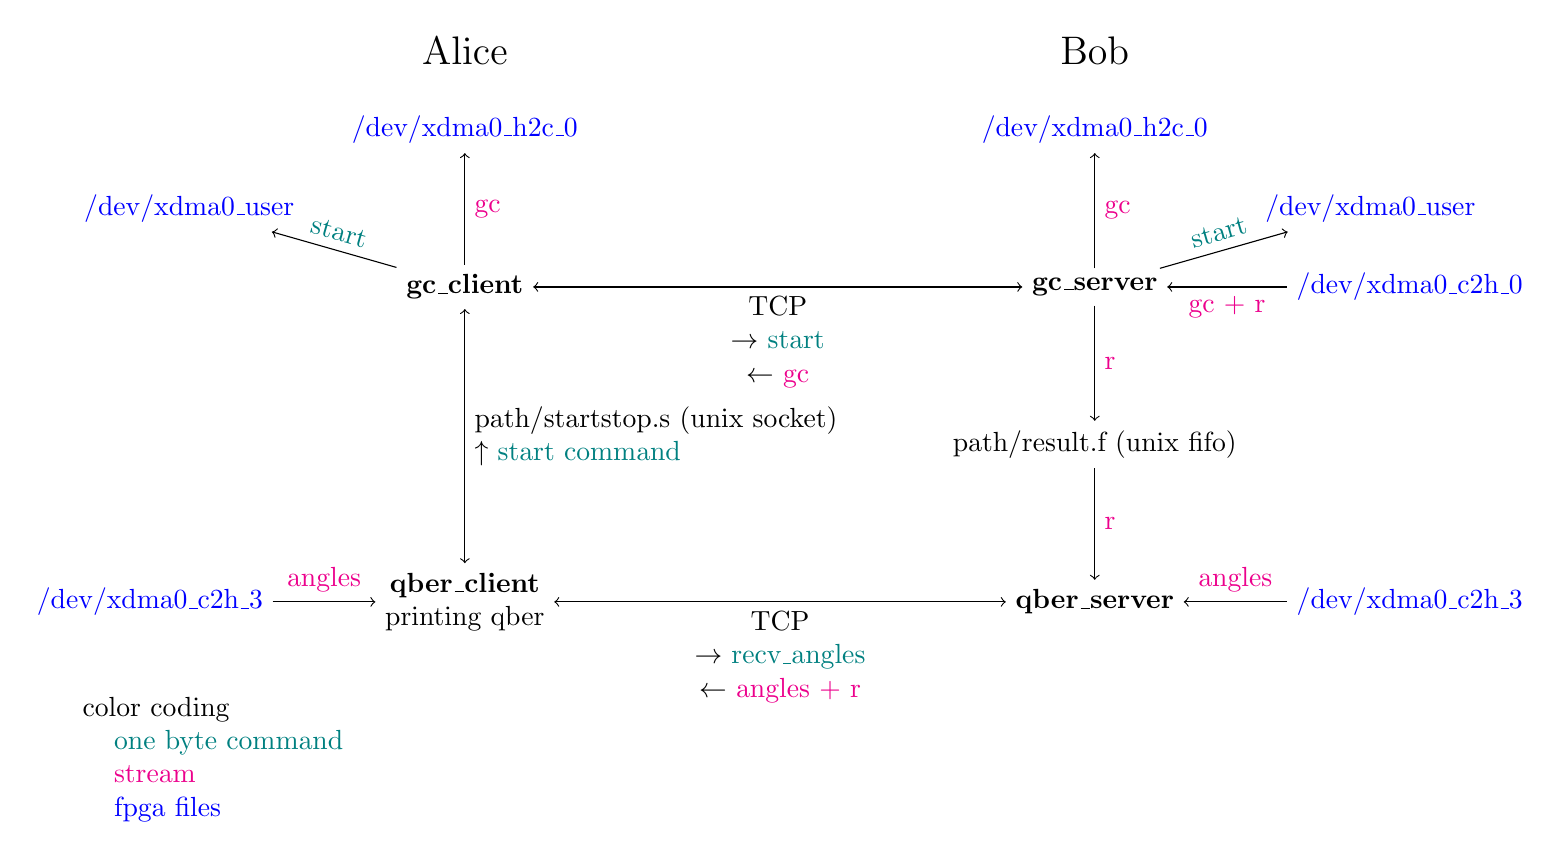
\begin{tikzpicture}
    \node at (0,2) {\Large Alice};
    \node at (8,2) {\Large Bob};

    \node[color=blue] (gcr) at (12, -1) {/dev/xdma0\_c2h\_0};
    \node[color=blue] (gcsb) at (8, 1) {/dev/xdma0\_h2c\_0};
    
    \node[color=blue] (gcsa) at (0, 1) {/dev/xdma0\_h2c\_0};
    \node[color=blue] (xdmaa) at (-3.5, 0) {/dev/xdma0\_user};
    \node[color=blue] (xdmab) at (11.5, 0) {/dev/xdma0\_user};

    \node(gcc) at (0,-1) {\textbf{gc\_client}};
    \node(gcs) at (8,-1) {\textbf{gc\_server}};

    \draw[<->] (gcc) -- (gcs) node(tcp)[below, midway, align=center]{TCP\\$\rightarrow$ \textcolor{teal}{start} \\$\leftarrow$ \textcolor{magenta}{gc}};

    
    \node(qberc) at (0,-5) [align=center] {\textbf{qber\_client}\\printing qber};
    \node(qbers) at (8,-5) {\textbf{qber\_server}};
    
    \node[color=blue] (aa) at (-4,-5) {/dev/xdma0\_c2h\_3};
    \draw[->] (aa) -- (qberc) node[midway, above]{\textcolor{magenta}{angles}};
    
    \node[color=blue] (ab) at (12,-5) {/dev/xdma0\_c2h\_3};
    \draw[->] (ab) -- (qbers) node[midway, above]{\textcolor{magenta}{angles}};
    
\draw[<->] (qberc) -- (qbers) node[below, midway, align=center]{TCP\\$\rightarrow$ \textcolor{teal}{recv\_angles}\\$\leftarrow$ \textcolor{magenta}{angles + r}};
    
    \draw[<->] (qberc) -- (gcc) node[midway, right, align=left]{path/startstop.s (unix socket) \\ $\uparrow$ \textcolor{teal}{start command}};

    \node (rf) at (8,-3) {path/result.f (unix fifo)};
    
    \draw[->] (gcs) -- (rf) node[midway, right]{\textcolor{magenta}{r}};
    \draw[->] (rf) -- (qbers) node[midway, right]{\textcolor{magenta}{r}};

    \draw[->] (gcr) -- (gcs) node[midway, below, align=left]{\textcolor{magenta}{gc + r}};
    \draw[->] (gcs) -- (gcsb) node[midway, right]{\textcolor{magenta}{gc}};
    \draw[->] (gcc) -- (gcsa) node[midway, right]{\textcolor{magenta}{gc}};
    
    \draw[->] (gcc) -- (xdmaa) node[midway, above, sloped]{\textcolor{teal}{start}};
    \draw[->] (gcs) -- (xdmab) node[midway, above, sloped]{\textcolor{teal}{start}};

    \node at (-3, -7) [align=left]{\hspace{-0.4cm}color coding\\\textcolor{teal}{one byte command}\\\textcolor{magenta}{stream}\\\textcolor{blue}{fpga files}};





\end{tikzpicture}


\end{document}







